%% 
%% Copyright 2019-2024 Elsevier Ltd
%% 
%% This file is part of the 'CAS Bundle'.
%% --------------------------------------
%% 
%% It may be distributed under the conditions of the LaTeX Project Public
%% License, either version 1.3c of this license or (at your option) any
%% later version.  The latest version of this license is in
%%    http://www.latex-project.org/lppl.txt
%% and version 1.3c or later is part of all distributions of LaTeX
%% version 1999/12/01 or later.
%% 
%% The list of all files belonging to the 'CAS Bundle' is
%% given in the file `manifest.txt'.
%% 
%% Template article for cas-dc documentclass for 
%% double column output.

\documentclass[a4paper,fleqn]{cas-dc}

% If the frontmatter runs over more than one page
% use the longmktitle option.

%\documentclass[a4paper,fleqn,longmktitle]{cas-dc}

%\usepackage[numbers]{natbib}
%\usepackage[authoryear]{natbib}
\usepackage[authoryear,longnamesfirst]{natbib}
\usepackage{cite}
\usepackage{amsmath,amssymb,amsfonts}
\usepackage{algorithmic}
\usepackage{graphicx}
\usepackage{textcomp}
\usepackage{xcolor}
\usepackage{float}
\usepackage{placeins}
\usepackage{tabularx}
\usepackage{multirow}
\usepackage{booktabs}
\usepackage{subcaption}

%%%Author macros
\def\tsc#1{\csdef{#1}{\textsc{\lowercase{#1}}\xspace}}
\tsc{WGM}
\tsc{QE}
%%%

% Uncomment and use as if needed
%\newtheorem{theorem}{Theorem}
%\newtheorem{lemma}[theorem]{Lemma}
%\newdefinition{rmk}{Remark}
%\newproof{pf}{Proof}
%\newproof{pot}{Proof of Theorem \ref{thm}}

\begin{document}
\let\WriteBookmarks\relax
\def\floatpagepagefraction{1}
\def\textpagefraction{.001}

% Short title
\shorttitle{FaceSM: Enhancing Transferable Face Attacks}    

% Short author
%\shortauthors{}  

% Main title of the paper
\title [mode = title]{FaceSM: Source-Separated and Mirror-Fused Objectives for Transferable Face Attacks}  

% Title footnote mark
% eg: \tnotemark[1]
%\tnotemark[1] 

% Title footnote 1.
% eg: \tnotetext[1]{Title footnote text}
%\tnotetext[1]{} 

% First author
%
% Options: Use if required
% eg: \author[1,3]{Author Name}[type=editor,
%       style=chinese,
%       auid=000,
%       bioid=1,
%       prefix=Sir,
%       orcid=0000-0000-0000-0000,
%       facebook=<facebook id>,
%       twitter=<twitter id>,
%       linkedin=<linkedin id>,
%       gplus=<gplus id>]

% \author[1]{}%[<options>]

% % Corresponding author indication
% \cormark[1]

% % Footnote of the first author
% \fnmark[1]

% % Email id of the first author
% \ead{}

% % URL of the first author
% \ead[url]{}

% % Credit authorship
% % eg: \credit{Conceptualization of this study, Methodology, Software}
% \credit{}

% % Address/affiliation
% \affiliation[1]{organization={},
%             addressline={}, 
%             city={},
% %          citysep={}, % Uncomment if no comma needed between city and postcode
%             postcode={}, 
%             state={},
%             country={}}

% \author[2]{}%[]

% % Footnote of the second author
% \fnmark[2]

% % Email id of the second author
% \ead{}

% % URL of the second author
% \ead[url]{}

% % Credit authorship
% \credit{}

% % Address/affiliation
% \affiliation[2]{organization={},
%             addressline={}, 
%             city={},
% %          citysep={}, % Uncomment if no comma needed between city and postcode
%             postcode={}, 
%             state={},
%             country={}}

% % Corresponding author text
% \cortext[1]{Corresponding author}

% % Footnote text
% \fntext[1]{}

% For a title note without a number/mark
%\nonumnote{}

% Here goes the abstract
\begin{abstract}
Face recognition systems remain vulnerable to transferable adversarial attacks, particularly in black-box settings where perturbations are crafted on surrogate models. Existing approaches typically optimize for target identity alignment in embedding space, but do not explicitly control residual source identity components, which can lead to entangled representations and limit transferability across models. This paper introduces FaceSM, an objective-level reformulation for transferable face attacks that addresses this limitation. The proposed method combines two complementary mechanisms: (i) a source-separated objective that jointly promotes alignment with the target identity while suppressing similarity to the source identity, and (ii) a mirror-fused embedding strategy that enforces consistency across horizontally flipped views to reduce sensitivity to view-specific artifacts induced by surrogate models.

FaceSM is integrated with five established attack backbones, including PGD, MI-FGSM, TI-FGSM, SI-NI-FGSM and MI-ADMIX-DI-TI, without modifying their optimization procedures. Experiments across four surrogate models and multiple unseen victim models on LFW, CelebA and VGGFace2 show consistent improvements in both breach rate and embedding-level impact. On a common victim pool, the average breach rate increases from 24.74\% to 29.88\%, with gains of up to 9.10 percentage points. External evaluation on RobFR confirms similar trends under black-box transfer. Further analysis of embedding trajectories and cross-model gradient alignment indicates that the proposed objective encourages more consistent optimization directions across models. These results highlight the importance of objective design in transferable attacks and suggest a simple yet effective direction for improving their generalization across face recognition systems.
\end{abstract}

% Use if graphical abstract is present
%\begin{graphicalabstract}
%\includegraphics{}
%\end{graphicalabstract}

% % Research highlights
% \begin{highlights}
% \item Proposes FaceSM, an objective reformulation for transferable face attacks.
% \item Introduces source separation to reduce identity entanglement in embeddings.
% \item Uses mirror-fused embeddings to improve view consistency across models.
% \item Shows consistent gains across attacks, models, and datasets with analysis.
% \end{highlights}


%\nocite{*}

% Keywords
% Each keyword is seperated by \sep
\begin{keywords}
 Adversarial Attacks\sep Face Verification\sep Transferability\sep Embedding Space\sep Biometrics 
\end{keywords}

\maketitle

\section{Introduction}
Deep face verification has become a core component of modern identity systems. It is widely used in mobile authentication, access control, remote onboarding, payment workflows and surveillance. Unlike closed-set classifiers, these systems map an image to a compact embedding and compare pairs using cosine similarity or a related distance measure \citet{taigman2014deepface,wang2018cosface}. A match is declared when the score crosses a threshold.

If an adversary can shift the embedding of one image while keeping the perturbation visually small, the final similarity score can cross the decision boundary. In face verification, the attack objective usually takes one of two forms. In an \emph{impersonation} setting, the adversary wants the source image to look similar to a target identity in embedding space. In a \emph{dodging} setting, the adversary wants to reduce similarity so that a legitimate match is rejected. Prior work has shown that both digital and physical attacks can succeed against face recognition pipelines \citet{sharif2016accessorize,goswami2018unravelling}.

The transfer setting is especially important in practice. Attackers rarely know the exact architecture, weights, preprocessing steps, or threshold calibration of the deployed verifier. The standard route is therefore to optimize the perturbation on a surrogate model and rely on transfer to an unseen victim. This is where many strong classification attacks become less reliable. Methods such as PGD \citet{madry2018towards}, MI-FGSM \citet{dong2018boosting}, TI-FGSM \citet{dong2019evading}, SI-NI-FGSM \citet{lin2020nesterov} and Admix \citet{wang2021admix} were developed largely with classifier decision surfaces in mind.

Adapting these methods to face verification typically involves replacing the classification loss with a cosine similarity objective, with little further modification. This limited adjustment leaves a meaningful gap. In particular, optimizing only for target alignment does not ensure that the adversarial representation departs sufficiently from the source identity. As a result, embeddings often retain residual source identity components, leading to mixed or entangled representations that can degrade transferability across models with different embedding geometries. A related problem is view dependence: single-view optimization tends to latch onto texture patterns tied to one specific presentation, making the resulting perturbation brittle when the victim applies a different alignment or normalization pipeline. This brittleness is compounded by the fact that horizontal flip augmentation is near-universal in face recognition training. Victim models such as Facenet and ArcFace are trained to treat a face and its mirror image as the same identity. As a result, they tend to average out view-specific artifacts that single-view perturbations rely on. Unlike other transformations such as rotation or vertical flipping, horizontal reflection preserves identity due to the bilateral symmetry of the human face \citet{farzmahdi2024emergence}.

This paper addresses both issues with \textbf{FaceSM}, an objective-level reformualtion that slots into any gradient-based iterative attack without touching its update rule, step schedule, or perturbation budget. FaceSM modifies what the optimizer is asked to do, rather than how it operates, by explicitly restructuring the objective to control embedding behavior during optimization. The first modification, \emph{source separation}, adds an explicit penalty for residual source identity alignment alongside the standard target-attraction term. Under the usual perturbation constraint, this keeps the image visually close to the source while driving its embedding away from the source identity manifold and toward the target. This formulation encourages a more direct and disentangled trajectory in embedding space, reducing ambiguity between identities. The second, \emph{mirror-fused optimization}, forms the embedding by averaging the encodings of the original image and its horizontal flip before renormalizing, grounding the objective in a view-consistent representation rather than a single potentially fragile one.

We pair FaceSM with five established attack backbones, namely PGD, MI-FGSM, TI-FGSM, SI-NI-FGSM and MI-ADMIX-DI-TI and evaluate across multiple surrogates and victim models on LFW, CelebA and VGGFace2. Every FaceSM-enhanced attack outperforms its vanilla counterpart on both breach rate and cosine impact on the main benchmark. An additional external validation on RobFR shows the same trend, with FaceSM consistently improving BIM, MIM, CIM and LGC under black-box transfer. Together, these results show that objective-level refinement can strengthen transferability without changing the underlying optimizer. The main contributions of this work are as follows:

\begin{itemize}
\item We propose \textbf{FaceSM}, an objective-level reformulation that improves transferability by explicitly reshaping embedding-space optimization, rather than modifying attack dynamics.
\item We introduce a \textbf{source-separated objective} that enforces joint target attraction and source repulsion, reducing identity entanglement and producing more transferable embedding trajectories.
\item We develop a \textbf{mirror-fused embedding strategy} that improves view consistency by integrating information from horizontally flipped inputs, reducing overfitting to a single representation and resulting in perturbations that generalize more effectively across models trained with augmentation-based invariances.
\item We conduct comprehensive experiments across multiple attack backbones, surrogate models, datasets, and an external benchmark, demonstrating consistent improvements in attack success and embedding-level impact. We further provide analysis of embedding trajectories and cross-model gradient alignment to offer insight into the mechanisms underlying improved transferability.
\end{itemize}

\section{Related Work}
\subsection{Transferable Adversarial Attacks}

Modern transfer attacks grew out of the observation that imperceptible perturbations cause large prediction errors in deep networks \citet{goodfellow2015explaining}. PGD established the multi-step baseline \citet{madry2018towards}, with subsequent work adding momentum \citet{dong2018boosting}, spatial smoothing \citet{dong2019evading}, scale invariance \citet{lin2020nesterov} and input mixing \citet{wang2021admix}. Input diversity methods, including DIM \citet{xie2019improving} and flipping-based augmentation \citet{fang2023improving}, reduce surrogate overfitting by exposing the optimizer to varied input presentations. These methods were designed for classification; face verification requires moving a pairwise similarity score across a threshold, a geometrically distinct objective that warrants a different treatment.

Recent work has further examined the factors that govern transferability across models. In particular, model alignment and loss landscape properties have been identified as key determinants of cross-model transfer, where perturbations that induce consistent update directions across architectures are more likely to generalize \citet{ma2024improving,wang2021enhancing}. Other studies have explored feature-space and representation-level attacks, showing that aligning perturbations with shared feature subspaces can improve transferability \citet{inkawhich2019feature}. These findings highlight that the design of the attack objective plays a central role in determining transfer performance.

\subsection{Adversarial Attacks on Face Verification}

Face recognition systems exhibit distinct structural properties and failure modes compared to standard classification models. Systems such as FaceNet and ArcFace represent faces through normalized embeddings rather than class probabilities \citet{schroff2015facenet,deng2019arcface}. The decision boundary is defined over pairs of representations rather than logits. This has led to a growing body of work on attacks that operate directly in embedding space. Vakhshiteh et al.\ examined the vulnerability of multiple face recognition models to standard gradient-based attacks \citet{vakhshiteh2021adversarial}, while Jia et al.\ proposed similarity-oriented gray-box objectives aligned with verification criteria \citet{wang2021similarity}. Transferability remains a central challenge. Differences in margins, input resolutions and feature geometries across models often cause perturbations crafted on one surrogate to degrade on unseen victims. FaceSM addresses this limitation by reshaping the objective rather than modifying the optimizer.

\subsection{Face-Specific Attack Objectives}

\begin{table*}[t]
\centering
\caption{Comparison of representative face adversarial attack methods. $F(\cdot)$: feature extractor; $\mathbf{x}^{a}$, $\mathbf{x}^{s}$, $\mathbf{x}^{t}$: adversarial, source, target embeddings.}
\label{tab:related}
\scriptsize
\resizebox{\textwidth}{!}{%
\begin{tabular}{@{}p{2.0cm} p{3.7cm} p{3.5cm} p{4.5cm}@{}}
\toprule
\textbf{Method} & \textbf{Objective} & \textbf{Approach} & \textbf{Impersonation / Dodging Behavior} \\
\midrule
DFANet (2020) \citet{zhong2020towards}
& $\min\displaystyle\sum_k\|F_{\theta_k}(\mathbf{x}^{a})-F_{\theta_k}(\mathbf{x}^{t})\|_2$
& Dropout on conv layers creates ensemble-like surrogate diversity.
& \textit{Imp:} pulls $\mathbf{x}^{a}$ toward $\mathbf{x}^{t}$ across surrogate copies. \textit{Dod:} no source-repulsion term; not supported. \\
\cmidrule(lr){1-4}
RobFR (2021) \citet{yang2020robfr}
& Imp: $\max\,\cos(F(\mathbf{x}^{a}),F(\mathbf{x}^{t}))$ \newline Dod: $\min\,\cos(F(\mathbf{x}^{a}),F(\mathbf{x}^{s}))$
& Benchmark applying iterative attacks to face verification; single-view objective.
& \textit{Imp:} cosine pull toward target. \textit{Dod:} cosine push from source; evaluated separately, not jointly. \\
\cmidrule(lr){1-4}
Adv-Makeup (2021) \citet{ijcai2021p173}
& $\min\;\mathcal{L}_{tgt} = 1 - \cos[F(\hat{\mathbf{x}}^{s}),\,F(\mathbf{x}^{t})]$\newline $\hat{\mathbf{x}}^{s}$: src. face + generated eye shadow
& Meta-learning over eye-shadow mask for black-box transfer.
& \textit{Imp:} cosine loss pulls toward target. \textit{Dod:} not formulated; no source term. \\
\cmidrule(lr){1-4}
Adv-Attr. (2022) \citet{jia2022adv}
& $\min\;[1-\cos(F(G_s(\mathbf{z}_i+\mathbf{n}_i)),\;F(\mathbf{x}^{t}))]$\newline
{\scriptsize $G_s$: StyleGAN generator; $\mathbf{z}_i$: attribute latent; $\mathbf{n}_i$: adv.\ noise}
& StyleGAN latent noise per attribute; importance-aware selection; Pareto optimization balances stealthiness and attack strength.
& \textit{Imp:} cosine pull toward target in semantic space. \textit{Dod:} not formulated. \\
\cmidrule(lr){1-4}
Sibling (2023) \citet{li2023sibling}
& $\mathcal{L}^*_{adv} = 1-\cos(f^*_a,\,f^*_v),\quad *\in\{F,A\}$
& Joint FR+AR cosine loss via hard-parameter sharing; JTMO+CTGS stabilise gradient fusion.
& \textit{Imp:} FR and AR branches pull toward target. \textit{Dod:} not formulated; no source suppression. \\
\cmidrule(lr){1-4}
\textbf{FaceSM (ours)}
& $\max\,\cos(F(\mathbf{x}^{a}),F(\mathbf{x}^{t}))-\lambda\cos(F(\mathbf{x}^{a}),F(\mathbf{x}^{s}))$
& Mirror-fused embedding; plug-in to any backbone.
& \textit{Imp:} $+\cos(\cdot,\mathbf{x}^{t})$ pulls toward target. \textit{Dod:} $-\lambda\cos(\cdot,\mathbf{x}^{s})$ repels from source. \textbf{Both jointly.} \\
\bottomrule
\end{tabular}}
\end{table*}

Table~\ref{tab:related} positions FaceSM against representative face attacks. DFANet introduces dropout on convolutional feature maps to create ensemble-like gradient diversity, but its objective remains target-driven. RobFR is a robustness benchmarking framework that applies iterative attacks to face verification without modifying their objectives. Adv-Makeup constrains perturbations to localized regions for improved stealth in black-box settings, while Adv-Attribute operates in a StyleGAN latent space with importance weighting. Sibling-Attack incorporates an auxiliary attribute recognition branch to enrich gradients through multi-task learning, but requires architectural modification and does not explicitly penalize source alignment. 

FaceSM differs from these approaches by keeping the attack backbone unchanged and introducing source suppression and mirror-fused consistency directly at the objective level.

In contrast to prior approaches that improve transferability through input transformations or optimization heuristics, our work focuses on the objective itself. We argue that transferability is fundamentally shaped by how the objective guides the embedding trajectory and propose a formulation that explicitly encourages disentangled and view-consistent representations.


\section{Problem Formulation and Threat Model}

We consider embedding-based face verification in a black-box transfer setting. Let $f(\cdot)$ denote a surrogate face model available to the attacker. Given a source image $x_s$ and a target image $x_t$, the attacker constructs an adversarial sample $x_{\mathrm{adv}}$ such that
\begin{equation}
\|x_{\mathrm{adv}} - x_s\|_\infty \leq \epsilon,
\end{equation}
with $\epsilon = 0.062$ in our experiments. The perturbation is clipped after each update so that the image remains within the valid input range.

The face model produces an embedding
\begin{equation}
e(x) = \frac{f(x)}{\|f(x)\|_2},
\end{equation}
and pairwise similarity is computed as
\begin{equation}
\mathrm{sim}(x_a, x_b) = e(x_a)^\top e(x_b).
\end{equation}

The attacker does not know the deployed victim model. Instead, optimization is performed on the surrogate and the resulting perturbation is evaluated on unseen victim verifiers. Two objectives are considered:
\begin{itemize}
\item \textbf{Impersonation}: increase similarity between the perturbed source and the target.
\item \textbf{Dodging}: reduce the similarity score so that a genuine pair falls below the victim threshold.
\end{itemize}

The key challenge is to produce a perturbation that is not tightly coupled to the surrogate model's exact embedding geometry.

\section{FaceSM Method}
\begin{figure*}
    \centering
    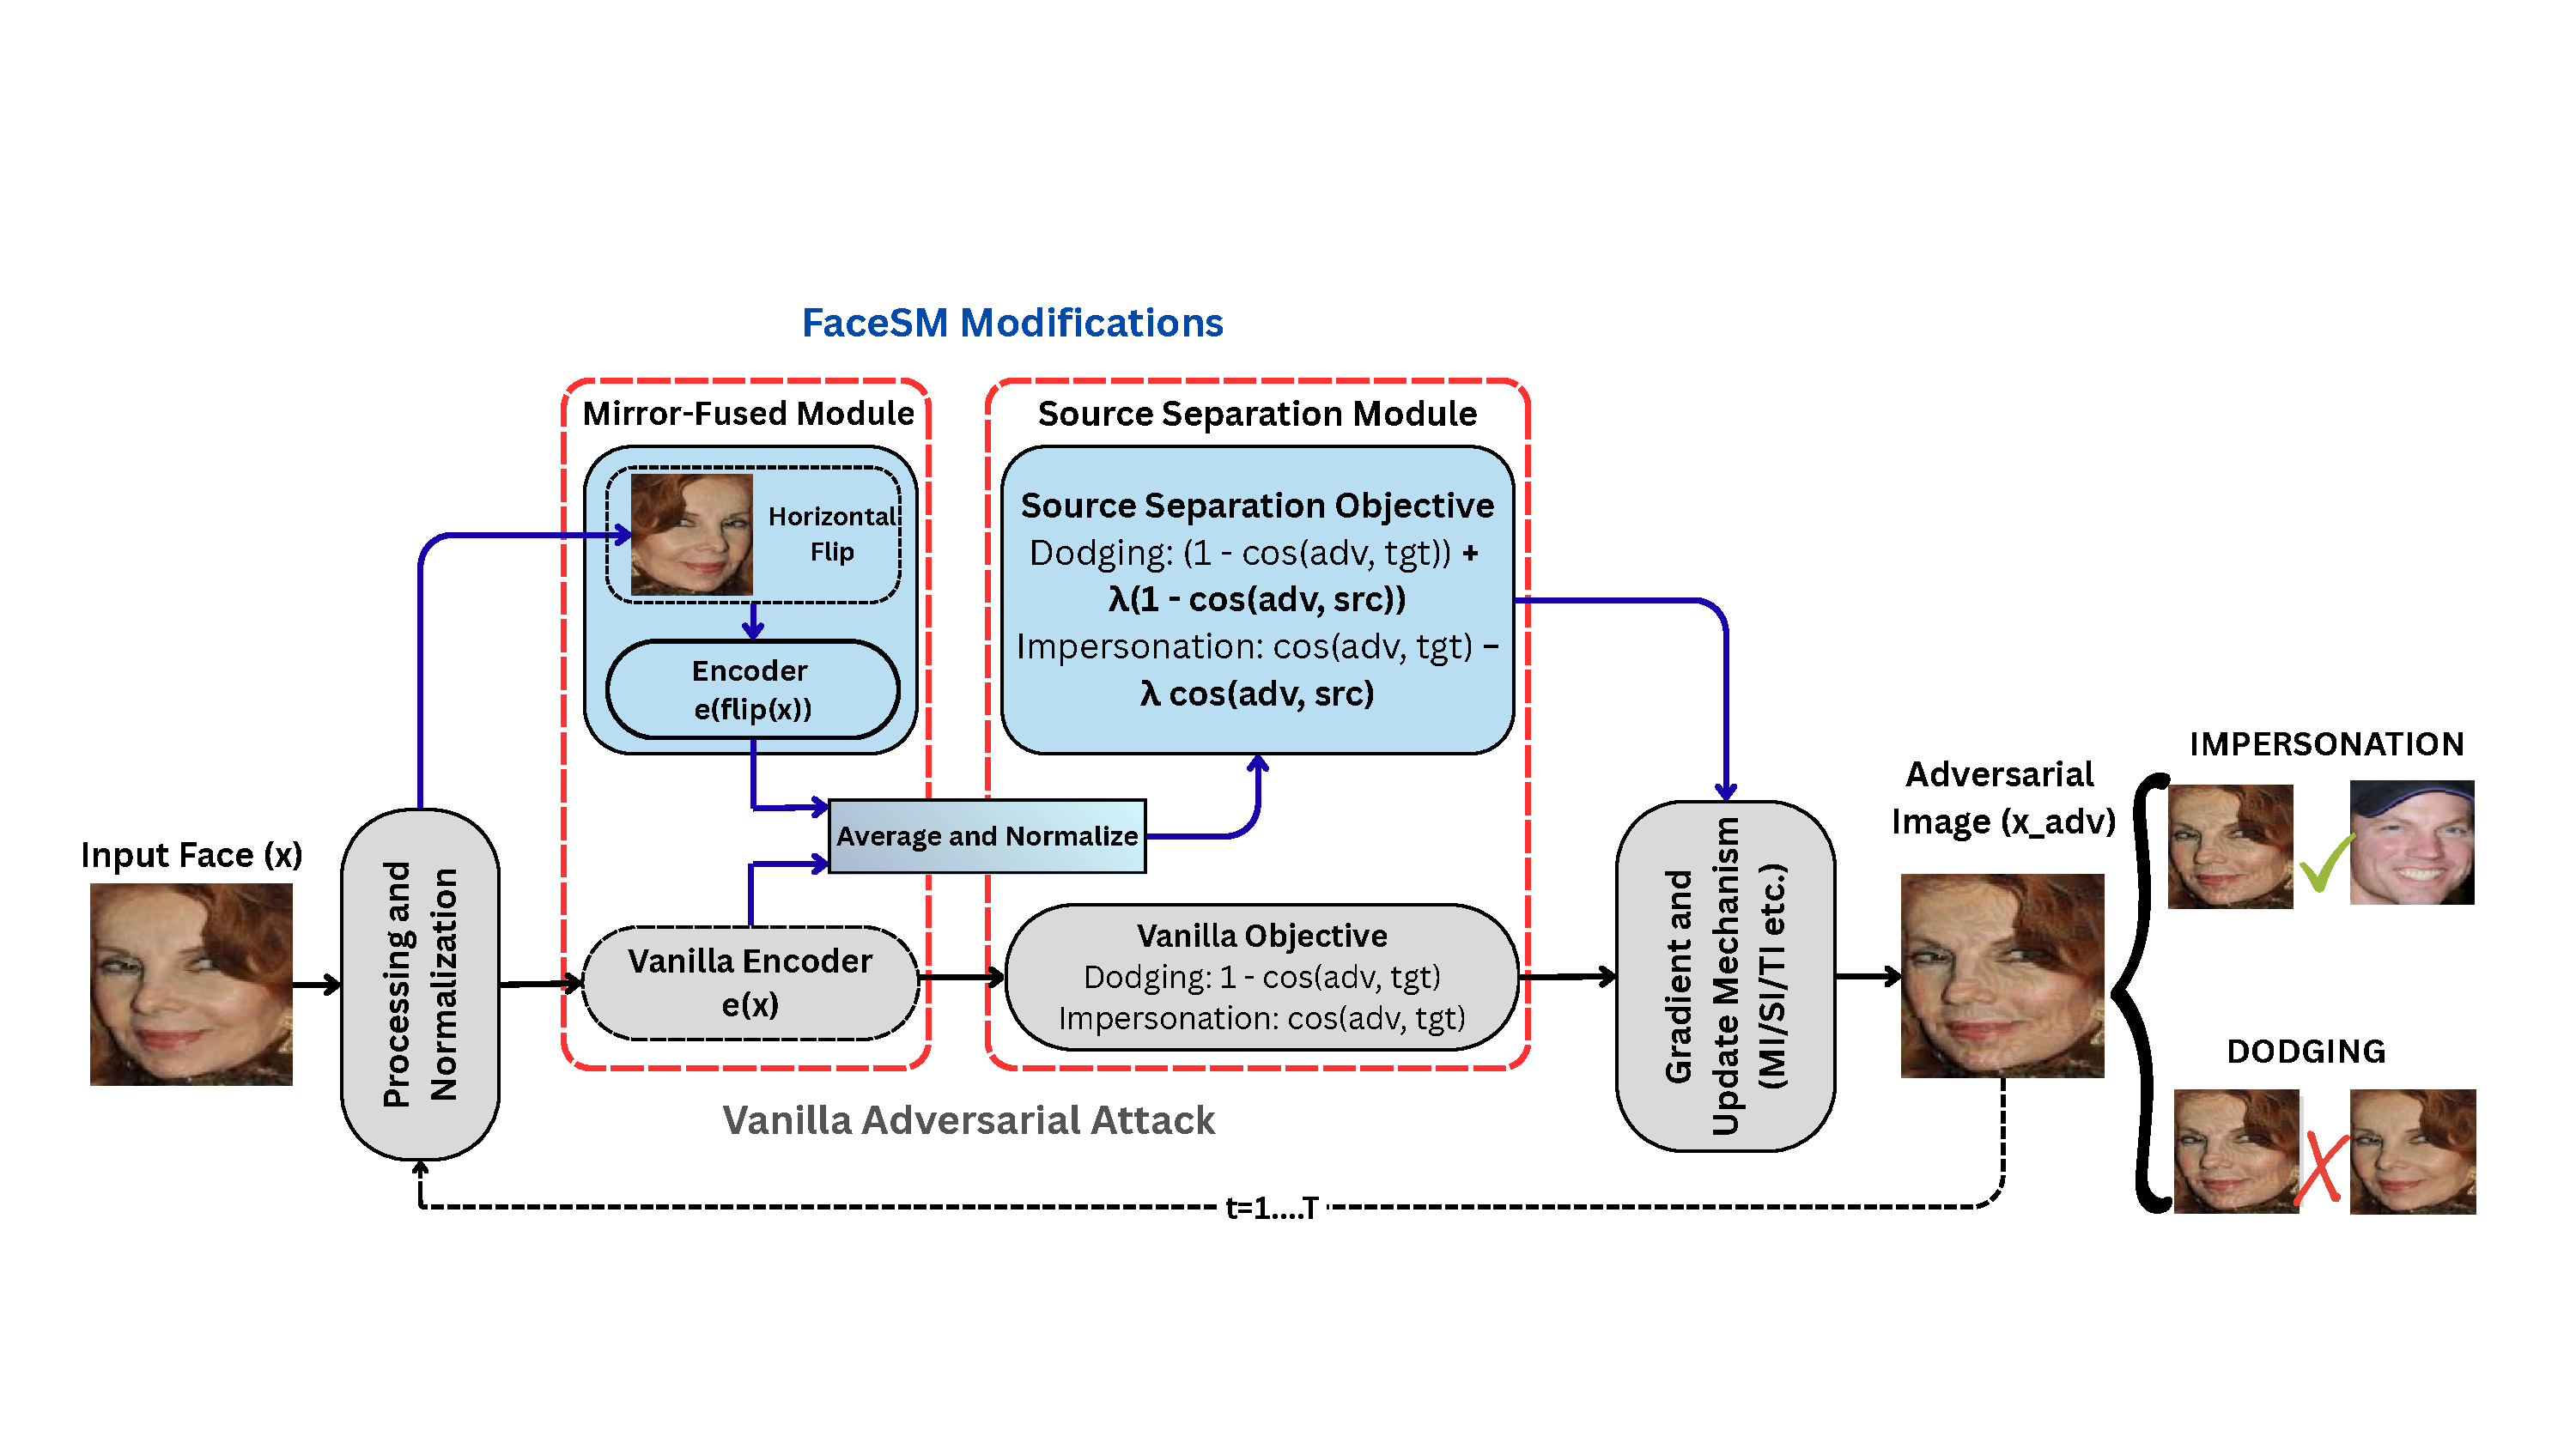
\includegraphics[width=\textwidth]{fig1_facesm-flowchart.pdf}
    \caption{FaceSM enhancement. Mirror-Fused Module averages embeddings of the original and horizontally flipped face to obtain a view-consistent representation. Source Separation Module augments the vanilla objective with a source-repulsion term.}
    \label{fig:facesm_overview}
\end{figure*}

\subsection{Overview}
FaceSM modifies the attack objective rather than the attack backbone. The motivation is intuitive. Target-only optimization is incomplete for impersonation. A perturbation can move an embedding closer to the target while still retaining strong source identity features. These residual components can limit how well the attack generalizes to unseen victim models.

A second issue is that single-view optimization tends to overfit to a specific representation of the face. This makes the resulting perturbation brittle when the victim applies different alignment or normalization. FaceSM addresses both issues through a source-separated objective and mirror-fused embedding, as illustrated in Figure~\ref{fig:facesm_overview}.

\subsection{Mirror-Fused Embedding}
Standard attacks optimize the embedding of a single input image, which anchors the optimization to one specific spatial configuration. However, face recognition models are typically trained with horizontal flip augmentation, encouraging embeddings that are invariant to left-right reflection. As a result, embeddings learned by such models implicitly average across mirrored views of the same identity. Perturbations optimized on a single view may exploit asymmetries that are not preserved by the victim model, leading to reduced transferability.

To mitigate this issue, FaceSM evaluates the objective on a mirror-fused embedding constructed from both the original image and its horizontally flipped version. Horizontal flip is used because it is a commonly employed transformation that preserves identity within the learned embedding manifold, unlike vertical flips or rotations which produce unrealistic facial structures.

Let \( e(x) \) denote the \( L_2 \)-normalized embedding of an image \( x \). The mirror-fused embedding is defined as
\begin{equation}
\tilde{e}(x) =
\frac{e(x) + e(\mathrm{flip}(x))}
{\left\| e(x) + e(\mathrm{flip}(x)) \right\|_2}.
\end{equation}
This fused representation reduces sensitivity to view-specific artifacts and provides a more stable optimization signal. It also acts as an implicit regularizer, discouraging overfitting to surrogate-specific representations.


\subsection{Source-Separated Objective}

The second component of FaceSM is source separation. The key idea is to explicitly suppress residual source identity alignment while maintaining visual similarity through the perturbation constraint. Rather than relying solely on target attraction, the objective encourages the adversarial embedding to move away from the source identity manifold.

Let \( \tilde{e}_s = \tilde{e}(x_s) \), \( \tilde{e}_t = \tilde{e}(x_t) \) and \( \tilde{e}(x) \) denote the mirror-fused embedding of the current adversarial sample. For impersonation, FaceSM uses the following objective:
\begin{equation}
\mathcal{L}_{\mathrm{FaceSM}}(x)
=
\cos\!\big(\tilde{e}(x),\,\tilde{e}_t\big)
-
\lambda \cos\!\big(\tilde{e}(x),\,\tilde{e}_s\big),
\end{equation}
where \( \lambda > 0 \) controls the strength of source suppression. The first term promotes alignment with the target identity, while the second term penalizes residual similarity to the source. This joint formulation encourages embeddings that are both target-oriented and disentangled from the source identity.

For dodging, we adopt a verification-oriented formulation:
\begin{equation}
\mathcal{L}_{\mathrm{dod}}(x)
=
\big(1 - \cos\!\big(\tilde{e}(x),\,\tilde{e}_t\big)\big)
+
\lambda \big(1 - \cos\!\big(\tilde{e}(x),\,\tilde{e}_s\big)\big).
\end{equation}

The additional term involving the target helps stabilize optimization by preventing degenerate solutions and maintaining a consistent embedding direction during updates.

\subsection{Integration with Existing Attacks}
FaceSM introduces two minimal modifications to existing gradient-based attacks. First, it replaces the standard loss with the source-separated objective. Second, it replaces the single-view embedding with the mirror-fused embedding. All other components of the attack, including the optimizer, momentum terms, projection steps and perturbation constraints, remain unchanged. This ensures that improvements can be attributed directly to the objective design, while preserving compatibility with a wide range of existing attack methods.

\section{Experimental Setup}

\subsection{Datasets}
We evaluate on three standard face verification benchmarks: LFW \citet{huang2008labeled}, CelebA \citet{liu2015deep} and VGGFace2 \citet{cao2018vggface2}. For each dataset, we use 1000 identity-controlled source--target pairs, with 500 samples per attack type. For impersonation, source and target images are drawn from different identities. For dodging, both images belong to the same identity. This construction ensures that each attack setting aligns with the corresponding verification objective. 

Each record consists of a source image, a target image, the dataset label and the attack type. All experiments are conducted on extracted and aligned face crops.

\subsection{Surrogate and Victim Models}
The benchmark uses four surrogate models: \textit{Facenet512}, \textit{GhostFaceNet}, \textit{ArcFace} and \textit{VGG-Face} \citet{schroff2015facenet,deng2019arcface,alansari2023ghostfacenets,parkhi2015deep}. Each surrogate is evaluated against a fixed pool of victim models, including \textit{Facenet512}, \textit{ArcFace}, \textit{GhostFaceNet}, \textit{VGG-Face} and \textit{IR-152}, covering diverse architectures and training objectives. The surrogate model is excluded from its own victim set to ensure a strict transfer setting.

Additionally, Facenet512 and Facenet share closely related architectures and embedding spaces. Cross-evaluation between them is therefore excluded to avoid inflated transfer estimates arising from representation similarity rather than true transferability.

\subsection{Attack Configuration}
All attacks share the same $\ell_\infty$ perturbation budget of $\epsilon = 0.062$ (equivalent to $16/255$ under normalized pixel scaling) and are run for 12 iterations. Both vanilla and FaceSM variants use identical settings, ensuring strictly paired comparisons. The source-separation coefficient is fixed at $\lambda = 0.20$, based on the sensitivity study in Section~\ref{subsec:lambda_sweep}. Random initialization is enabled for PGD-based methods.

We attach FaceSM to five baselines namely PGD, MI-FGSM, TI-FGSM, SI-NI-FGSM and MI-ADMIX-DI-TI and keep all hyperparameters identical between vanilla and FaceSM variants. Decision thresholds are model and dataset-specific and are computed on a large validation set within the evaluation pipeline. All thresholds are calibrated at a false accept rate (FAR) of 0.1\%.

FaceSM introduces minimal computational overhead, requiring one additional embedding evaluation per iteration due to the mirror-fused representation, while leaving the optimization procedure and hyperparameters unchanged.

\subsection{Evaluation Metrics}
We report two metrics. \textbf{Breach rate (B)} measures the fraction of cases in which the adversarial similarity score exceeds the victim decision threshold. \textbf{Impact (Imp)} measures the signed change in similarity score induced by the attack: for impersonation it is $s_{\mathrm{adv}} - s_{\mathrm{clean}}$ and for dodging it is $s_{\mathrm{clean}} - s_{\mathrm{adv}}$. Breach rate reflects decision-level success, while impact captures the magnitude of change in the embedding space. 

\subsection{External RobFR Validation}
To verify that the observed improvements are not specific to our evaluation pipeline, we conduct external validation using the RobFR benchmark \citet{yang2020robfr}. FaceSM is integrated with four black-box iterative attacks from RobFR: BIM, MIM, CIM and LGC. We use \textit{ArcFace} as the surrogate and \textit{FaceNet-VGGFace} as an unseen victim and evaluate on 300 LFW pairs provided by the benchmark for each attack setting. Both impersonation and dodging are considered.

Although this setup is narrower than the main benchmark, it provides an external validation under an independent framework and confirms that the same transfer gains persist in a black-box setting.


\section{Results and Discussion}
We evaluate FaceSM on five attack backbones, four surrogate models and three datasets. We report the main benchmark first, then RobFR external validation, followed by ablation and sensitivity analyses. All aggregate metrics use the common victim pool of Facenet, ArcFace, GhostFaceNet, VGG-Face and IR-152, excluding the surrogate from its own victim set.

\subsection{Main Benchmark Results}

\subsubsection{Overall Pairwise Comparison}

Table~\ref{tab:pairwise_split} reports the attack-wise comparison under impersonation and dodging settings. FaceSM improves both breach rate and impact across all attack backbones in both scenarios. The gains are consistently larger under dodging, where the source-separation term aligns more directly with the verification objective by explicitly reducing source similarity.

Performance improvements vary across backbones. MI-FGSM and SI-NI-FGSM benefit the most, showing substantial increases in both metrics. In contrast, MI-ADMIX-DI-TI exhibits smaller gains, suggesting that stronger baselines leave less room for objective-level improvement. This trend is consistent with the ablation results in Table~\ref{tab:ablation_components}, where mirror-fused optimization provides the dominant standalone gain, while source separation contributes an additional complementary improvement.

\begin{table}[t]
\centering
\caption{Attack-wise comparison for impersonation and dodging settings on the common victim pool.}
\label{tab:pairwise_split}
\setlength{\tabcolsep}{3pt}
\renewcommand{\arraystretch}{1.15}
\footnotesize
\begin{tabularx}{\columnwidth}{Xccccc}
\toprule
Attack & V-B (\%) & SM-B (\%) & V-Imp & SM-Imp & $\Delta$B (pp) \\
\midrule
\multicolumn{6}{c}{\textbf{Impersonation}} \\
\midrule
MI-ADMIX-DI-TI & 12.32 & \textbf{13.97} & 0.0713 & \textbf{0.0780} & +1.65 \\
MI-FGSM        & 12.67 & \textbf{16.94} & 0.0715 & \textbf{0.0863} & +4.27 \\
PGD            &  6.84 & \textbf{ 9.91} & 0.0476 & \textbf{0.0604} & +3.06 \\
SI-NI-FGSM     & 16.45 & \textbf{21.40} & 0.0837 & \textbf{0.1012} & +4.95 \\
TI-FGSM        & 10.19 & \textbf{13.56} & 0.0611 & \textbf{0.0732} & +3.37 \\
\midrule
\multicolumn{6}{c}{\textbf{Dodging}} \\
\midrule
MI-ADMIX-DI-TI & 39.69 & \textbf{43.21} & 0.1944 & \textbf{0.2130} & +3.53 \\
MI-FGSM        & 41.34 & \textbf{50.44} & 0.2017 & \textbf{0.2421} & +9.10 \\
PGD            & 26.05 & \textbf{31.52} & 0.1183 & \textbf{0.1532} & +5.47 \\
SI-NI-FGSM     & 45.26 & \textbf{54.13} & 0.2199 & \textbf{0.2570} & +8.87 \\
TI-FGSM        & 32.73 & \textbf{39.40} & 0.1614 & \textbf{0.1939} & +6.68 \\
\bottomrule
\end{tabularx}
\end{table}

\subsubsection{Surrogate-wise Behavior}

Figure~\ref{fig:breach_combined} (a) compares the average breach rate of the vanilla attacks and FaceSM across the four surrogate models. FaceSM improves all surrogates. The largest gain is obtained with ArcFace, whose breach rate rises from 19.98\% to 26.79\%. Facenet512 and VGG-Face also improve clearly, by +4.59 and +5.77 percentage points, respectively. GhostFaceNet remains the most difficult surrogate overall, but FaceSM still raises its breach rate from 9.39\% to 12.96\%. These results indicate that the method is effective across diverse embedding spaces, while the size of the gain still depends on the transfer strength of the underlying surrogate.

\begin{figure*}
\centering

\begin{minipage}{0.48\textwidth}
    \centering
    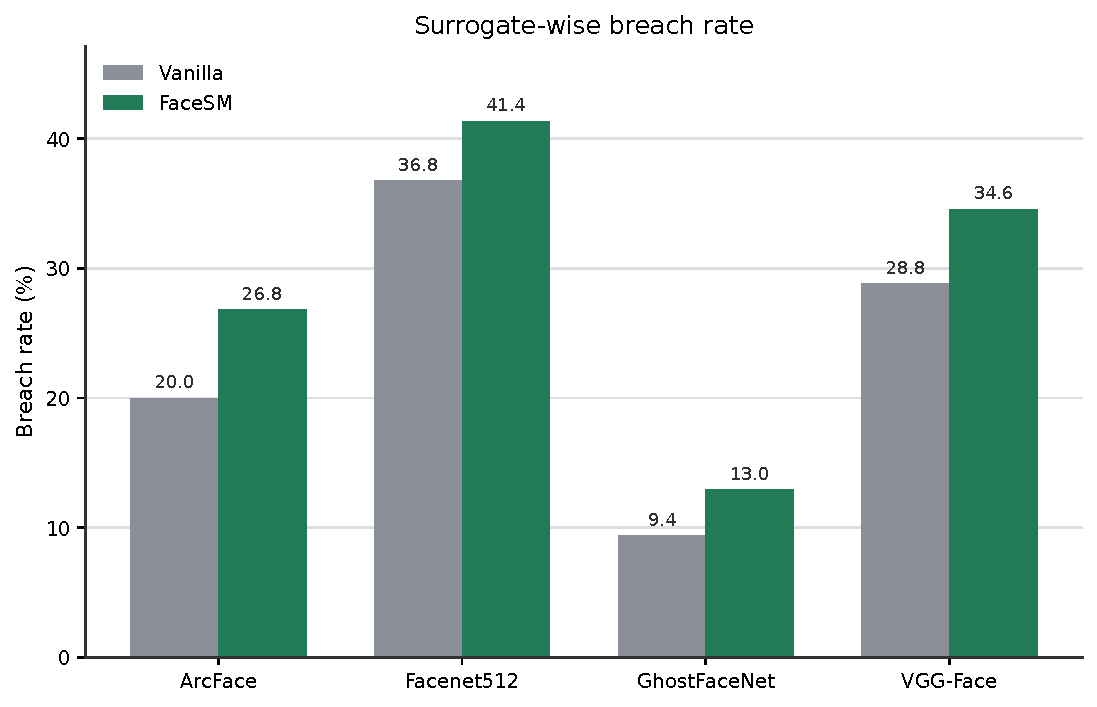
\includegraphics[width=\linewidth]{fig2a_surrogate_breach.pdf}
    {\footnotesize (a) Surrogate models}
\end{minipage}
\hfill
\begin{minipage}{0.48\textwidth}
    \centering
    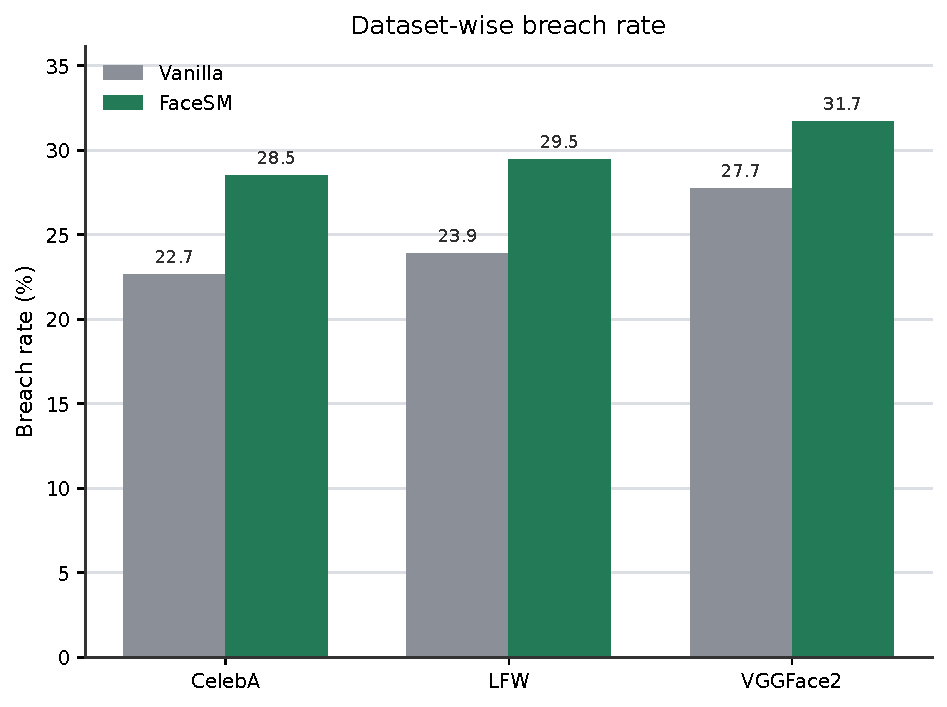
\includegraphics[width=\linewidth]{fig2b_dataset_breach.pdf}
    {\footnotesize (b) Datasets}
\end{minipage}

\caption{Average breach rate of vanilla attacks and FaceSM across (a) surrogate models and (b) datasets.}
\label{fig:breach_combined}
\end{figure*}

\subsubsection{Dataset-wise Generalization}

Figure~\ref{fig:breach_combined} (b) shows the same comparison across datasets. The improvement is consistent on CelebA, LFW and VGGFace2, with breach-rate gains of +5.86, +5.55 and +4.00 percentage points, respectively. VGGFace2 shows the smallest margin, which is expected given its higher pair difficulty and broader identity variation, but the improvement remains clear. This consistency across datasets suggests that FaceSM improves the transfer objective itself rather than benefiting from a specific data distribution.

The improvements are consistent across all evaluated configurations, with no negative transfer cases observed, indicating robustness of the proposed objective formulation.

\subsection{Cross Model Transferability Analysis}

\begin{table*}[t]
\centering
\caption{Cross-model breach-rate improvement ($\Delta$B, percentage points) for valid surrogate--victim transfer pairs. Positive values indicate better transfer under FaceSM. Self-transfer pairs are excluded and the Facenet512-Facenet pair is omitted as a same-family case.}
\label{tab:cross_model}
\setlength{\tabcolsep}{5pt}
\renewcommand{\arraystretch}{1.15}
\begin{tabular}{lccccccc}
\toprule
\textbf{Attacker} & \textbf{ArcFace} & \textbf{Facenet} & \textbf{Facenet512} & \textbf{GhostFaceNet} & \textbf{IR152} & \textbf{VGG-Face} & \textbf{Avg. $\Delta$B} \\
\midrule
ArcFace      & --    & +10.24 & +9.30  & +4.80 & +7.94 & +7.70 & +8.00 \\
Facenet512   & +4.68 & --     & --     & +3.06 & +5.02 & +5.62 & +4.59 \\
GhostFaceNet & +5.11 & +3.09  & +3.29  & --    & +2.69 & +2.93 & +3.42 \\
VGG-Face     & +8.16 & +13.42 & +12.96 & +4.34 & +4.82 & --    & +8.74 \\
\midrule
\textbf{Avg. by victim} & +5.98 & +8.92 & +8.52 & +4.07 & +5.12 & +5.42 & \textbf{+6.27} \\
\bottomrule
\end{tabular}
\end{table*}

We evaluate cross-model transfer on surrogate--victim pairs where attacks are generated on one model and tested on a different, unseen model. Self-transfer pairs are excluded and we also omit the Facenet512 $\rightarrow$ Facenet case because these two models belong to the same family and do not represent a meaningful cross-model transfer setting. Under this protocol, the broader common victim set yields 19 valid transfer pairs.

Table~\ref{tab:cross_model} shows that FaceSM improves breach rate in all 19 evaluated pairs. The gain ranges from \textbf{2.69} to \textbf{13.42} percentage points, with a mean improvement of \textbf{+6.27} percentage points. Impact also improves consistently across all pairs, with gains ranging from \textbf{0.0107} to \textbf{0.0669} and a mean increase of \textbf{0.0318}.

Transferability still varies across surrogates. Facenet512 remains the strongest baseline surrogate overall, with average breach rate rising from \textbf{36.76\%} to \textbf{41.36\%}. VGG-Face shows the largest average improvement, increasing from \textbf{34.02\%} to \textbf{42.76\%} (\textbf{+8.74} pp). ArcFace also benefits strongly, improving from \textbf{18.52\%} to \textbf{26.52\%}. GhostFaceNet remains the weakest baseline surrogate, but FaceSM still improves all of its valid transfer pairs, with gains between \textbf{2.69} and \textbf{5.11} percentage points.

On the victim side, IR152 remains the most robust model, with the lowest average vanilla breach rate (\textbf{10.86\%}), but it still rises to \textbf{15.97\%} under FaceSM. The largest gains are observed on the Facenet-family victims when the surrogate comes from a different family, especially VGG-Face $\rightarrow$ Facenet (\textbf{+13.42} pp), VGG-Face $\rightarrow$ Facenet512 (\textbf{+12.96} pp) and ArcFace $\rightarrow$ Facenet (\textbf{+10.24} pp). Overall, these results show that the proposed objective-level refinements reliably strengthen adversarial transferability across diverse face-verification architectures.



\subsection{External Validation on RobFR}
\label{subsec:robfr_validation}

Table~\ref{tab:robfr_validation} shows that the same overall pattern remains. Under dodging, FaceSM improves all four attacks by a clear margin. BIM increases from 8.33\% to 16.67\% breach rate, MIM from 13.33\% to 22.00\%, CIM from 13.67\% to 24.00\% and LGC from 15.67\% to 22.67\%. Under impersonation, the absolute gains are smaller but still consistent: BIM rises from 1.33\% to 3.00\%, MIM from 2.33\% to 5.00\%, CIM from 2.33\% to 4.67\% and LGC from 2.00\% to 5.00\%. The victim-side similarity score also moves in the expected direction in every case, decreasing for dodging and increasing for impersonation. Averaged across the four RobFR attacks, breach rate rises from 12.75\% to 21.33\% under dodging and from 2.00\% to 4.42\% under impersonation. Although this RobFR setting is smaller in scope than our main benchmark, it supports the same conclusion: FaceSM improves transferability when attached to established iterative attacks and the gain is not specific to our custom pipeline.

\begin{table}[t]
\centering
\caption{External validation on RobFR using ArcFace as surrogate.}
\label{tab:robfr_validation}
\setlength{\tabcolsep}{3pt}
\renewcommand{\arraystretch}{1.15}
\small
\begin{tabularx}{\columnwidth}{lccccc}
\toprule
Attack & V-B (\%) & SM-B (\%) & $\Delta$B (pp) & V-Score & SM-Score \\
\midrule
\multicolumn{6}{c}{\textbf{Dodging}} \\
\midrule
BIM & 8.33 & \textbf{16.67} & +8.33 & 0.6152 & \textbf{0.5630} \\
MIM & 13.33 & \textbf{22.00} & +8.67 & 0.5776 & \textbf{0.5313} \\
CIM & 13.67 & \textbf{24.00} & +10.33 & 0.5727 & \textbf{0.5276} \\
LGC & 15.67 & \textbf{22.67} & +7.00 & 0.5733 & \textbf{0.5369} \\
\midrule
\multicolumn{6}{c}{\textbf{Impersonation}} \\
\midrule
BIM & 1.33 & \textbf{3.00} & +1.67 & 0.0975 & \textbf{0.1302} \\
MIM & 2.33 & \textbf{5.00} & +2.67 & 0.1230 & \textbf{0.1538} \\
CIM & 2.33 & \textbf{4.67} & +2.33 & 0.1281 & \textbf{0.1565} \\
LGC & 2.00 & \textbf{5.00} & +3.00 & 0.1323 & \textbf{0.1548} \\
\bottomrule
\end{tabularx}
\end{table}

\subsection{Ablation Study}

We isolate the contribution of each component using SI-NI-FGSM as the backbone, reporting overall averages on the common victim pool (Table~\ref{tab:ablation_components}). Mirror-fused optimization provides the larger standalone gain, increasing the breach rate from 28.98\% to 33.24\%, indicating that view-consistent gradients are a major contributor to improved transferability. Source separation yields a smaller but consistent improvement (30.00\%), suggesting that suppressing residual source alignment alone is less effective when the optimization remains tied to a single-view representation. Combining both components achieves the best performance (33.98\%, 0.1751), yielding the largest overall improvement. The gain over either component alone suggests that the two mechanisms address complementary aspects of the transfer problem.
\begin{table}[t]
\centering
\caption{Ablation of FaceSM components using SI-NI-FGSM. MF: mirror-fused optimization. SS: source separation.}
\label{tab:ablation_components}
\small
\begin{tabular}{lccc}
\toprule
Configuration & Breach (\%) & Impact & $\Delta$ (\%) \\
\midrule
Vanilla        & 28.98 & 0.1581 & -- \\
SS Only        & 30.00 & 0.1597 & +1.02 \\
MF Only        & 33.24 & 0.1730 & +4.26 \\
FaceSM (SS+MF) & \textbf{33.98} & \textbf{0.1751} & \textbf{+5.00} \\
\bottomrule
\end{tabular}
\end{table}

\subsection{Sensitivity to the Source-Separation Weight}
\label{subsec:lambda_sweep}
\begin{figure}
\centering
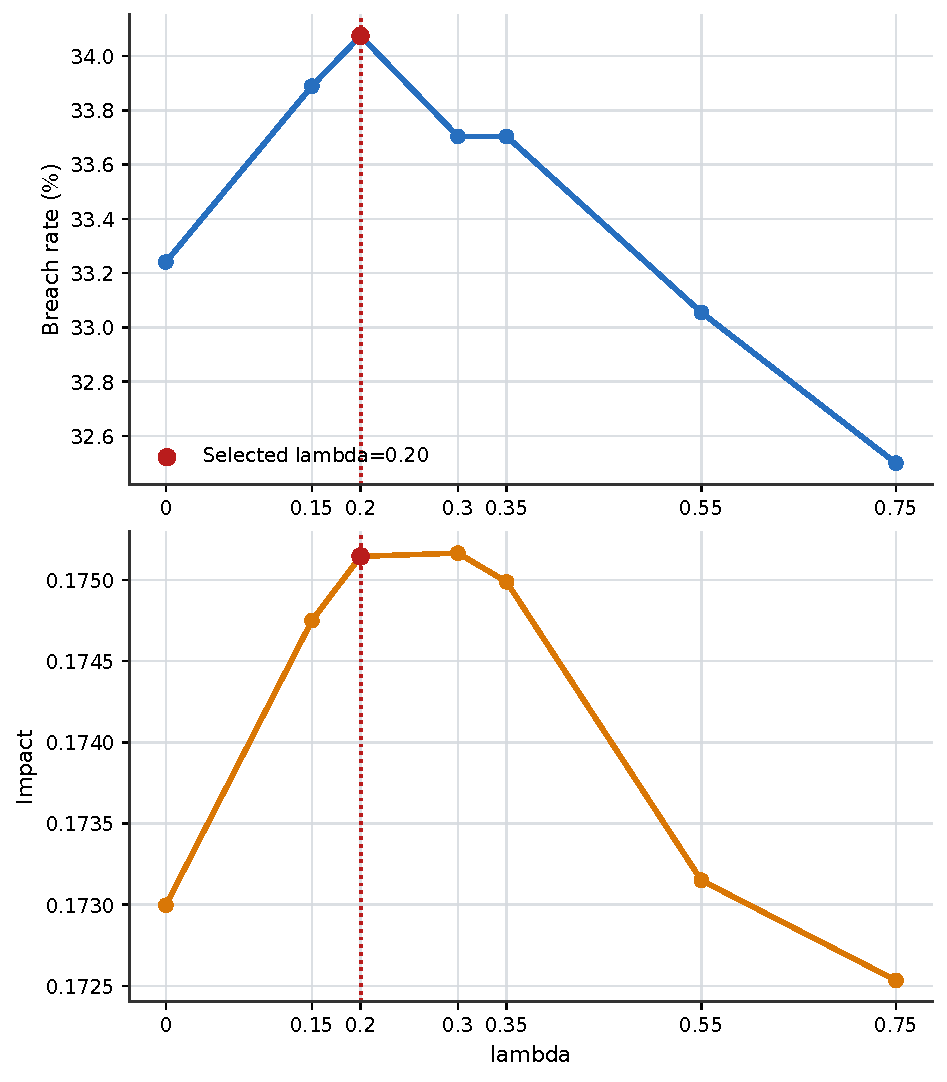
\includegraphics[width=0.95\linewidth]{fig3_lambda_sweep_vertical.pdf}
\caption{Sensitivity of FaceSM to the source-separation coefficient $\lambda$. Top: average breach rate. Bottom: average impact.}
\label{fig:lambda_sweep}
\end{figure}
Figure~\ref{fig:lambda_sweep} shows the sensitivity of FaceSM variant of SI-NI-FGSM to the source-separation coefficient $\lambda$. Moving away from $\lambda=0$ improves performance and the method remains stable over a moderate range. Averaged across Facenet512 and GhostFaceNet, breach rate is highest at $\lambda=0.20$, while impact varies only slightly from 0.20 to 0.35. Larger values, such as 0.55 and 0.75, reduce both metrics, indicating that overly strong source suppression begins to conflict with target alignment. Based on this trend, we set $\lambda=0.20$ throughout.

\subsection{Mechanistic Analysis of Transferability Improvement}
To understand why FaceSM improves transfer, we examine two behavioral signatures of the optimization: how adversarial embeddings evolve relative to source and target identities across iterations and how consistently the resulting gradients align across models. We demonstrate that FaceSM changes optimization dynamics by improving cross-model gradient consistency.

\subsubsection{Embedding Trajectory Analysis}

Figure~\ref{fig:embedding_trajectory} tracks cosine similarity to both target and source identities across iterations for SI-NI-FGSM and its FaceSM variant. In both cases, similarity to the target increases steadily, indicating that source separation does not interfere with target attraction.

The difference appears in the evolution of source similarity. The vanilla attack maintains a relatively high level of alignment with the source identity throughout optimization. In contrast, FaceSM rapidly suppresses source similarity within the first few iterations and maintains it at a low level thereafter. This behavior reflects the effect of the source-separation term, which penalizes residual source alignment at every step. As a result, the embedding follows a more direct trajectory toward the target identity, rather than remaining in an intermediate region influenced by both source and target. This more decisive movement through the embedding space contributes to improved transferability.

\begin{figure}
\centering
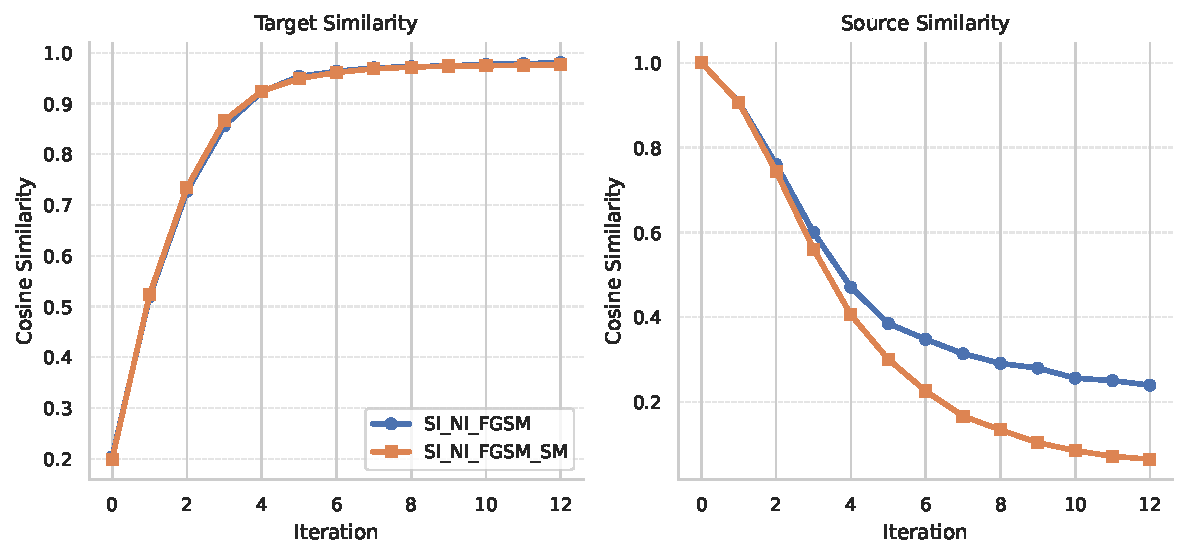
\includegraphics[width=0.95\linewidth]{fig4_embedding_trajectory.pdf}
\caption{Embedding trajectory comparison between vanilla SI-NI-FGSM and FaceSM variant under impersonation attack.}
\label{fig:embedding_trajectory}
\end{figure}


\begin{figure*}
\centering

\begin{minipage}{0.48\textwidth}
    \centering
    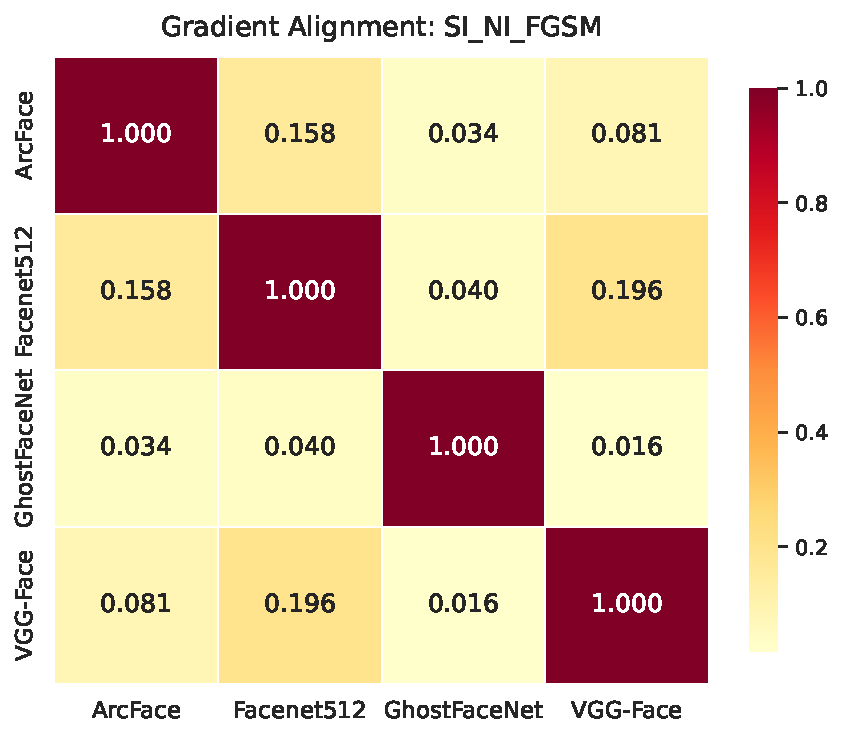
\includegraphics[width=\linewidth]{fig5a_sini_alignment.pdf}
    \\
    {\footnotesize (a) Vanilla alignment}
\end{minipage}
\hfill
\begin{minipage}{0.48\textwidth}
    \centering
    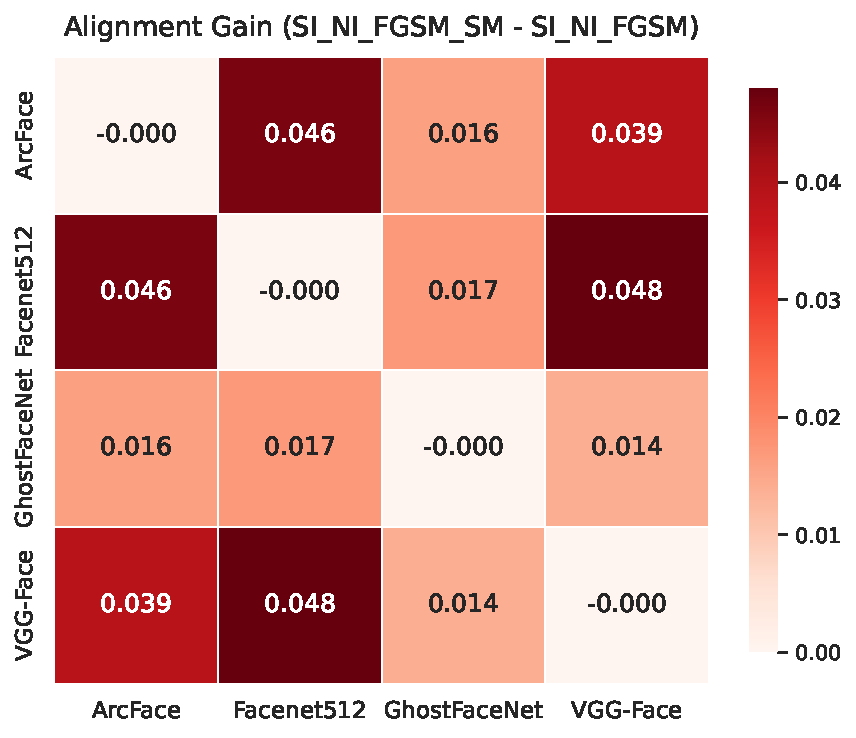
\includegraphics[width=\linewidth]{fig5b_alignment_gain.pdf}
    \\
    {\footnotesize (b) Alignment gains}
\end{minipage}

\caption{Cross-model gradient alignment.}
\label{fig:grad_align}
\end{figure*}

\subsubsection{Gradient Alignment Analysis}
Transferability depends on whether the update direction computed on a surrogate model remains meaningful when evaluated on a different model. If two models produce similar gradient directions for the same input, perturbations optimized on one model are more likely to transfer successfully to the other. To quantify this effect, we compute pairwise cosine similarity between input-space gradients of the attack loss across surrogate models. The left heatmap in Figure~\ref{fig:grad_align} shows that gradients produced by vanilla SI-NI-FGSM are nearly orthogonal across model pairs, indicating that each model induces a largely independent update direction. As a result, perturbations optimized on one surrogate carry limited transferable signal.
FaceSM alters this behavior. By grounding the objective in a view-consistent and source-disentangled embedding, the resulting gradients become more aligned across models. The gain matrix shows consistent increases in alignment across all model pairs, with no negative entries. The effect is most pronounced for the Facenet512–VGG-Face pair (+0.048) and ArcFace–Facenet512 (+0.046). These results indicate that FaceSM encourages update directions that are more consistent across models. This improved alignment provides a plausible explanation for the observed gains in transferability.

\subsection{Implications for Real-World Face Recognition Systems}

The observed improvements in transferability have direct implications for face recognition systems deployed in real-world environments. In practical scenarios, such systems are often integrated into broader decision-making pipelines, including mobile authentication, access control, remote identity verification, and surveillance. These deployments typically rely on fixed decision thresholds and are expected to operate reliably under diverse input conditions. The results of this work suggest that adversarial perturbations generated on surrogate models can generalize across architectures more effectively than previously assumed, increasing the feasibility of black-box attacks.

This raises concerns regarding the robustness of embedding-based verification. Since decisions are based on similarity scores rather than explicit class labels, relatively small but structured shifts in embedding space can lead to incorrect outcomes without noticeable visual distortion. The proposed formulation illustrates how residual identity information and view-dependent biases can be systematically exploited, indicating that current evaluation practices may underestimate vulnerability in cross-model settings.

These observations highlight the need for robustness assessments beyond single-model or white-box assumptions. In particular, defense strategies should consider objective-level manipulation and transfer-driven attack scenarios that do not require precise knowledge of the deployed model. Incorporating cross-model evaluation and embedding-space analysis into validation protocols may therefore be necessary for reliable deployment in security-sensitive applications.

\section{Conclusion and Future Scope}
This work demonstrates that objective design plays a central role in determining the transferability of adversarial attacks in embedding-based face verification systems. By introducing source separation and mirror-fused embedding, FaceSM provides a simple yet effective reformulation that consistently improves transfer performance without modifying optimization dynamics. Across five attack families, four surrogates, three datasets and multiple unseen victims, every FaceSM variant outperforms its vanilla counterpart on both breach rate and impact. The gains are largest for simpler baselines and smallest where the vanilla attack already incorporates heavy transfer-enhancement, but remain positive throughout. The same trend also appears under external validation on RobFR, where FaceSM improves BIM, MIM, CIM and LGC under black-box transfer. These results suggest that refining what the surrogate is asked to optimize is a straightforward and consistently effective path to better transfer. 

Future work could explore whether these modifications remain effective under physical-world constraints or when combined with surrogate ensembles. Beyond that, adaptive weighting of the source-repulsion term, alternative view-fusion strategies beyond horizontal flip and evaluation under adversarial defenses and commercial APIs are natural next steps toward a more complete understanding of objective-level refinements for face attack transferability.

\section{Declaration of generative AI and AI-assisted technologies in the manuscript preparation process}
During the preparation of this work, the authors used ChatGPT for minor language editing and refinement. After using this tool, the authors reviewed and edited the content as needed and take full responsibility for the content of the published article.

\section{Data Availability}
Code, experiment scripts, and supplementary materials supporting this study are available through the following anonymous repository:
\texttt{https://github.com/AItruste/ml-study-23}. The underlying LFW, CelebA, and VGGFace2 datasets are public benchmarks and should be obtained from their official sources, subject to their respective licensing terms. Raw dataset images are therefore not redistributed as part of this repository.

%% The Appendices part is started with the command \appendix;
%% appendix sections are then done as normal sections
%% \appendix


% To print the credit authorship contribution details
%\printcredits

%% Loading bibliography style file
%\bibliographystyle{model1-num-names}
\bibliographystyle{cas-model2-names}

% Loading bibliography database
\bibliography{cas-refs}

% Biography
%\bio{}
% Here goes the biography details.
%\endbio

%\bio{pic1}
% Here goes the biography details.
%\endbio

\end{document}

